\documentclass[aspectratio=169]{SUSTechBeamer}
\usetheme{Malmoe}
\title{Journey to \LaTeX}
\subtitle{An introduction to the typesetting system}
\author[Solo \textit{et al.}]{Han~Solo\inst{1}
    \and Luke~Skywalker\inst{2}
    \and Darth~Vadar\inst{3}
}
\institute[SUSTech]{\inst{1}Southern University of Science and Technology
    \and \inst{2} Jedi Academy
    \and \inst{3} Galatic Empire
}
\date[2000 Winter]{January 1st, 2000}
\begin{document}
\setbeamertemplate{headline}{}
\setbeamertemplate{footline}{}
\begin{frame}
    \titlepage
\end{frame}

\setbeamertemplate{footline}[\defaultfoot]
\begin{frame}
    \tableofcontents
\end{frame}
\setbeamertemplate{headline}[\defaulthead]

\section{Introduction}
\subsection{Introduction}
\begin{frame}{Introduction}
  \begin{itemize}
    \item Welcome to the presentation on \LaTeX!
    \item \LaTeX is a powerful typesetting system widely used in academic and scientific writing.
    \item It offers precise control over document formatting and produces high-quality output.
    \item In this presentation, we will explore the features and benefits of \LaTeX.
  \end{itemize}
\end{frame}

\subsection{Importance}
\begin{frame}{Importance of \LaTeX}
    \begin{columns}
        \begin{column}{0.5\textwidth}
            \begin{figure}[h]
                \centering
                \includegraphics[width=\linewidth]{demo_fig/pdffig.pdf}
                \caption{caption of the figure}
                \label{fig:fig1}
            \end{figure}
        \end{column}
    \begin{column}{0.5\textwidth}
        \begin{itemize}
          \item \LaTeX plays a crucial role in various academic and scientific fields,including:
          \item Research papers, theses, and dissertations
          \item Presentations, posters, and conference proceedings
          \item Mathematical and scientific documents
          \item Journals and publications
          \item By using \LaTeX, authors can focus on content creation while ensuring professional and standardized document formatting.
        \end{itemize}
    \end{column}
\end{columns}
\end{frame}

\subsection{Overview}
\begin{frame}{Overview of the Presentation Structure}\
    \begin{columns}
        \begin{column}{0.4\textwidth}
            \begin{figure}[h]
                \centering
                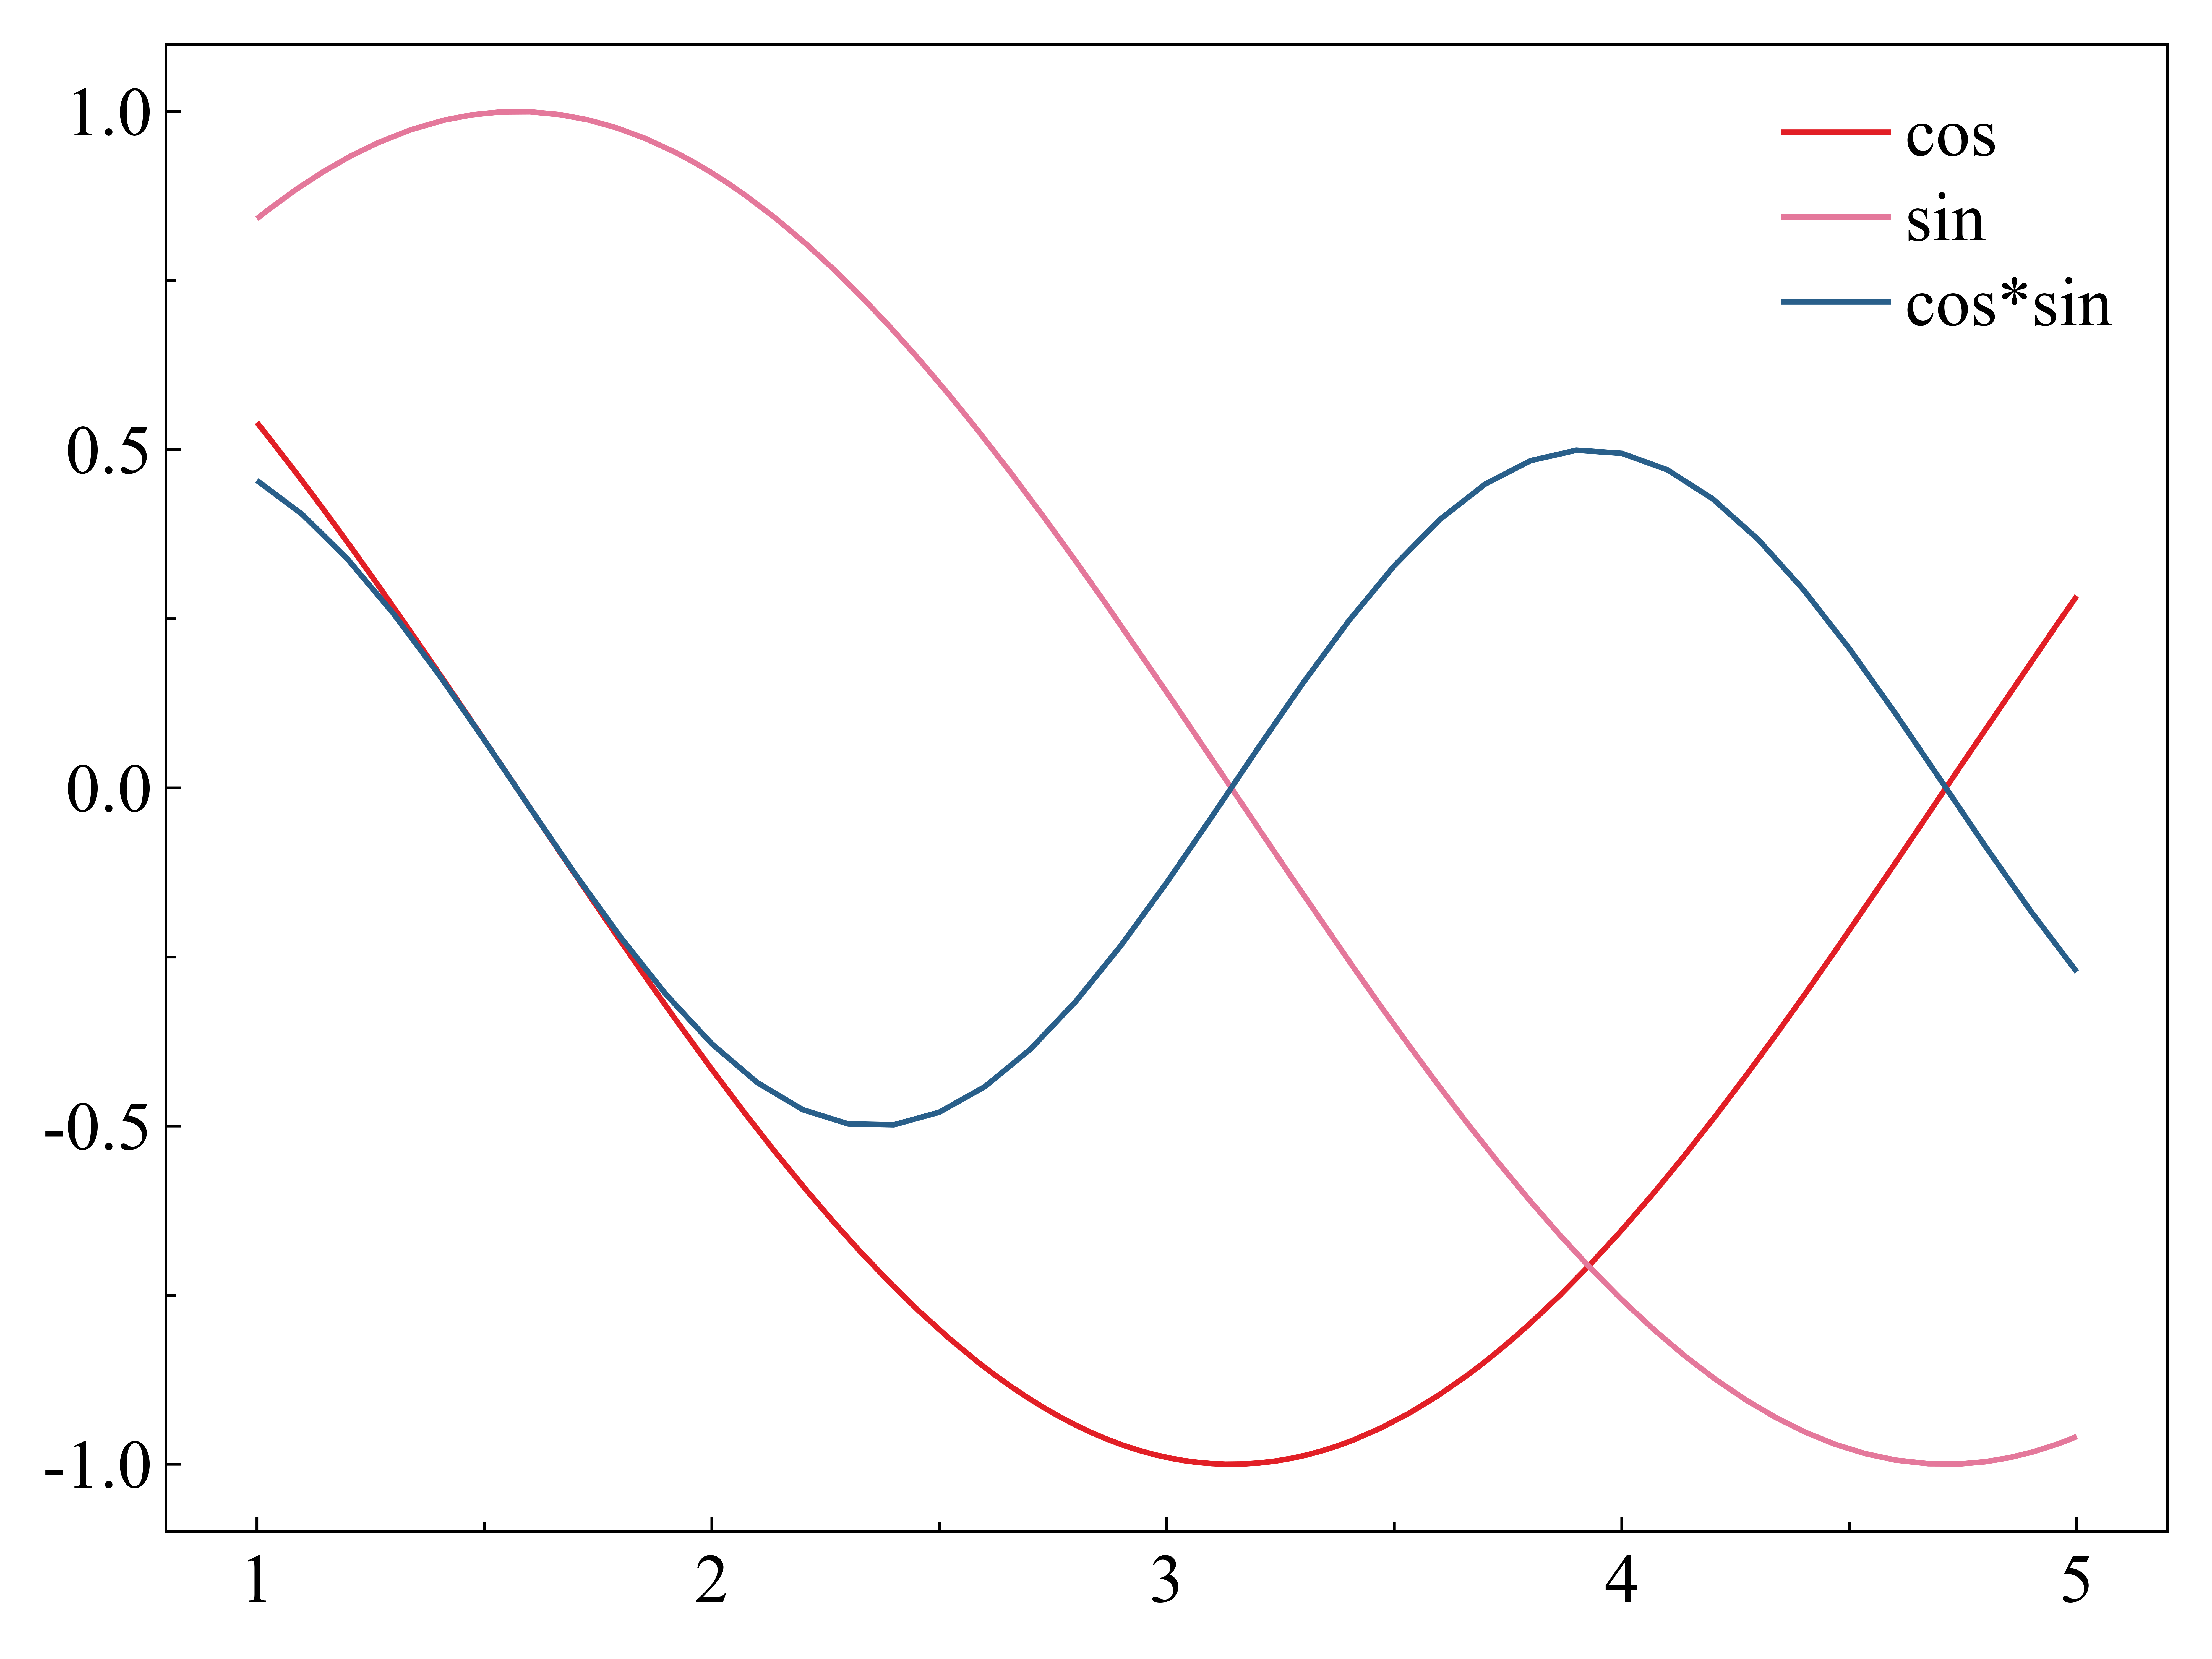
\includegraphics[width=\linewidth]{demo_fig/pngfig.png}
                \caption{the second fig}
                \label{fig:fig2}
            \end{figure}
        \end{column}
        \begin{column}{0.6\textwidth}
        \begin{itemize}
            \item In this presentation, we will cover the following topics:
            \item What is \LaTeX?
            \item Getting Started with \LaTeX
            \item Document Structure and Formatting
            \item Customizing Documents with Packages and Templates
            \item Advanced Features and Tips
            \item Troubleshooting and Resources
        \end{itemize}
    \end{column}
\end{columns}
\end{frame}

\section{What is \LaTeX?}

\subsection{Definition and History}
\begin{frame}{Definition and History of \LaTeX}
    \begin{columns}
        \begin{column}{0.6\textwidth}
  \LaTeX is a typesetting system widely used for the production of technical and scientific documents. It was developed by Leslie Lamport in the early 1980s, based on the TeX typesetting system created by Donald Knuth.

  \LaTeX provides a set of macros and commands that simplify document preparation and allow precise control over formatting. It follows a markup language approach where the content and structure of the document are separate from its presentation. \LaTeX is open source and available for multiple platforms, making it highly accessible to users.
        \end{column}
        \begin{column}{0.4\textwidth}
            \begin{align}
                \p{\rho}{t}+\rho\p{u_i}{x_i}&=0\\
                \p{u_i}{t}+u_j\p{u_i}{x_j}&=\frac{1}{\rho}\p{\sigma_{ij}}{x_j}+f_i
            \end{align}
        \end{column}
    \end{columns}
\end{frame}

\subsection{Comparison}
\begin{frame}{Comparison between \LaTeX and Word Processors}
  Unlike traditional word processors (e.g., Microsoft Word), \LaTeX focuses on the logical structure of the document rather than its visual appearance. Word processors are often WYSIWYG (What You See Is What You Get), while \LaTeX follows a WYSIWYM (What You See Is What You Mean) approach.

  \LaTeX offers superior typesetting capabilities, especially for mathematical equations, complex layouts, and large documents. Collaboration and version control are easier with \LaTeX, as plain text source files can be stored in version control systems like Git. However, the learning curve for \LaTeX is steeper compared to word processors due to its markup language nature.
\end{frame}

\subsection{Advantages}
\begin{frame}{Advantages of Using \LaTeX}
    \begin{itemize}
      \item High-quality output: \LaTeX produces professional-looking documents with precise typography and line-breaking algorithms.
      \item Cross-referencing and referencing tools: \LaTeX automatically handles numbering and referencing of sections, equations, figures, and tables.
      \item Mathematical typesetting: \LaTeX excels at typesetting complex mathematical equations and symbols.
      \item Consistent formatting: \LaTeX templates ensure consistent styles throughout the document and can be easily modified.
      \item Focus on content: \LaTeX separates content creation from formatting, allowing authors to focus on the actual writing.
      \item Large user community and extensive resources: \LaTeX has a vast user base, active community support, and numerous online resources.
    \end{itemize}
\end{frame}


\section{Conclusion}

\subsection{Summary}
\begin{frame}{Summary of Key Points}
In this presentation, we explored the following key points about LaTeX:

\begin{itemize}
    \item LaTeX is a powerful typesetting system widely used in academic and scientific writing.
    \item It offers precise control over document formatting and produces high-quality output.
    \item LaTeX follows a markup language approach, separating content from presentation.
    \item LaTeX provides superior typesetting capabilities, especially for mathematical equations and complex layouts.
    \item Collaboration and version control are facilitated by LaTeX's plain text source files.
    \item LaTeX offers consistent formatting, cross-referencing, and extensive resources.
\end{itemize}
\end{frame}

\subsection{Exploration and Practice}
\begin{frame}{Encouraging Further Exploration and Practice}
\begin{itemize}
    \item LaTeX has a steep learning curve, but with practice, it becomes a valuable skill for academic and scientific writing.
    \item Experiment with different LaTeX packages and templates to enhance your document's visual appeal and functionality.
    \item Join online LaTeX communities and forums to seek help, share knowledge, and discover new possibilities.
    \item Continuously improve your LaTeX skills by exploring advanced features, such as custom macros and document classes.
    \item Keep up with the latest developments in the LaTeX ecosystem, including new packages and updates to existing ones.
    \item Embrace LaTeX as a tool that empowers you to create professional and visually appealing documents.
\end{itemize}
\end{frame}

\subsection{Q\&A Session}
\begin{frame}{Q\&A Session}
    Now, I would be happy to answer any questions you may have about LaTeX or any topics covered in this presentation.

    Feel free to ask about specific LaTeX features, best practices, or any challenges you may be facing.
\end{frame}

\end{document}